\documentclass[a4paper,10pt]{article}
\usepackage[utf8x]{inputenc}
\usepackage{amsmath}
\usepackage{amssymb}
\usepackage{bbm}
\usepackage[pdftex]{graphicx}
\usepackage{epstopdf}

\graphicspath{{./Figs/}}
%opening
\title{ Lecture 3: Quantifiers and Sets}

\begin{document}
\maketitle
\section{ Quantifiers in Theorems}
\textbf{Definition 3.1.1 (Universal Quantifiers).} The universal quantifier is a symbol which expresses that the statement is true  ``for all '' or `` any'' $x$, for e.g., a statement such as `` $(\forall x\in U)P(x)$'' $\Longleftrightarrow$ If $x\in U$ then $P(x)$ is true.  

\textbf{Proof strategy.} To prove a statement with universal quantifiers to be true, prove that the statement is true for any arbitrary $x \in U$ then this will be true for any $x\in U$. 

Example: Prove that $f(n) = n^2+n+41$ is prime $\forall n\in\{0,\ldots, 39\}$ 

\textbf{Proof strategy by contradiction.} Pick a $y\in U$ and suppose that $P(y)$ then using argumentation arrive at a contradiction.

\textbf{Definition 3.1.2 (Existential Quantifiers).} The existential quantifier $\exists$ is a symbol which represents that there exists some element for which statement $P(x)$ is true. 

\textbf{Proof strategy.} To prove a statement such as \emph{$(\exists x \in U)P(x) $} one need to find some $x_0\in U$ such that $P(x_0)$ holds.
\section{Tips for Writing Mathematics}
\begin{enumerate}
 \item A written proof should stand on its own.
 \item Write precisely and clearly.
 \item Prove what is appropriate.
 \item Be careful with saying things are ``obvious''. 
 \item Use full sentences and correct grammar, for e.g., $x=z^2$ could be written as `` the variable $x$ equals to the square of variable $z$''.
 \item Use ``='' sign properly.
 \item Define all symbols and terms you make up. 
 \item Break up a long proof into steps. 
 \item Distinguish formal vs informal writing.
 \item Miscellaneous Tips
 \begin{enumerate}
  \item No mathematical symbols after punctuation.
  \item Don't use logical symbols such as $ \vee , \wedge ,\exists , \forall , \implies $ for words in proof.
  \item Use equal sign only in equations.
  \item Use consistent notation.
  \item Display long formulas (or short important ones) on their own lines. 
  \item Avoid colons.
  \item Capitalize names such as Theorem 2.3, Lemma 1.7.  
 \end{enumerate}
\end{enumerate}
\section{Sets}
\subsection{Basic Definitions.}
\textbf{Definition 3.3.1 (Sets).} Set is a collection of objects. Objects contained in the set are called the ``elements'' of the set. If $\mathcal{A}$ is a set, and $a$ is an element of the set $\mathcal{A}$, we write $a\in \mathcal{A}$. If $a$ is not contained in $\mathcal{A}$, then we write $a\notin\mathcal{A}$. A set is written as $\{a,b,c,\ldots,e\}$, here ordering is irrelevant. 

\textbf{Important sets.}
\begin{enumerate}
 \item Set of natural numbers $\mathbbm{N} =\{1,2,\ldots\}$
 \item Set of integers $\mathbbm{Z} =\{\ldots,-3,-2,-1,0, 1,2,\ldots\}$
 \item Set of rational numbers $\mathbbm{Q}$
 \item Set of real numbers $\mathbbm{R}$
 \item set of whole numbers $\mathbbm{N}_0$
  \item Empty set $\phi$ 
\end{enumerate}

\textbf{Example 3.2} Let $S=\{n\in \mathbbm{Z}| n \text{ is a perfect square}\}$, then 
\begin{eqnarray*}
 S&=&\{n\in \mathbbm{Z}| n =k^2\text{ for some} k\in \mathbbm{Z}\}\\
 &=&S=\{n\in \mathbbm{Z}| \text{ is a perfect square } k\in \mathbbm{Z} \text{ such that } n=k^2 \}
\end{eqnarray*}
\textbf{Definition 3.3.2 (Intervals).}

\textbf{Definition 3.3.2.1 (Open Interval).} An open interval is defined as follows $$(a,b):= \{x\in \mathbbm{R}: a<x<b\}$$

\textbf{Definition 3.3.2.2 (Closed Interval).} A closed interval is defined as $$[a,b]:= \{x\in \mathbbm{R}: a\leq x\leq b\}$$

\textbf{Definition 3.3.2.3 (Half-open Interval).} A half-open interval is defined as  $$[a,b):= \{x\in \mathbbm{R}: a<x\leq b\}$$

\textbf{Definition 3.3.2.4 (Infinite Interval).} An infinite interval is defined as $$[a,\infty):= \{x\in \mathbbm{R}: a\leq x\}.$$ Other infinite intervals can be $(a,-\infty)$, $(-\infty,b]$, $(-\infty,\infty)=\mathbbm{R}$

\textbf{Remark 1:} $+\infty$ and $-\infty$ are not real numbers.

\textbf{Remark 2:} Dummy variables cannot be used outside without redefining them.
\subsection{Relation between Sets.}
 Let $\mathcal{A}$ and $\mathcal{B}$ be sets
 
 \textbf{Definition 3.3.3 (Subset)} We say that $\mathcal{A}$ is a ``subset'' of $\mathcal{B}$ if $x\in \mathcal{A}$ implies $x\in \mathcal{B}$, and is denoted by $\mathcal{A}\subset \mathcal{B}$. This is shown in following figure 
 
\begin{figure}[!h]
\centering
 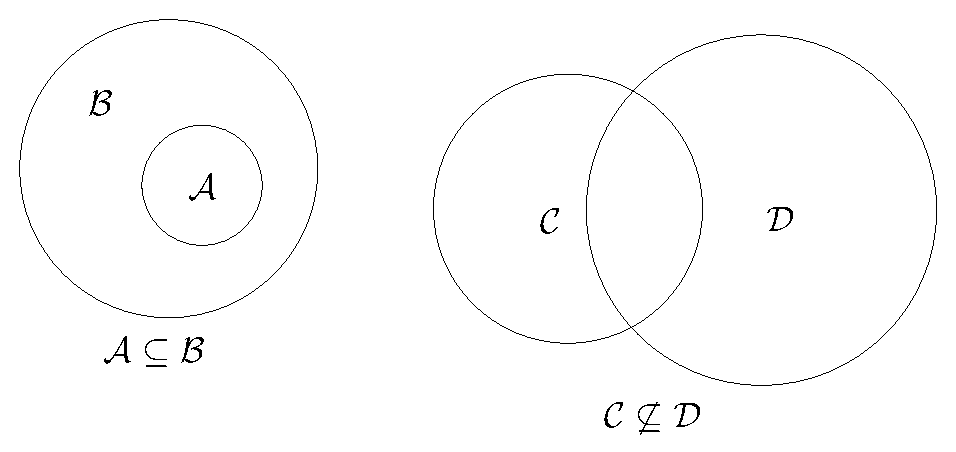
\includegraphics[height=1.0in]{fig33.eps}
\end{figure}
In other words, we can say that $\mathcal{A}\subseteq \mathcal{B}$ if $\forall x [(x\in \mathcal{A}) \rightarrow (x\in\mathcal{B})]$. While, we say that $\mathcal{A}\nsubseteq\mathcal{B}$ if $\exists$ $x$ such that $[x\in\mathcal{A}\rightarrow x\not\in\mathcal{B}]$.

\textbf{Lemma 3.1} Let $\mathcal{A},\mathcal{B}$ and $\mathcal{C}$ be sets then following is true
\begin{enumerate}
 \item $\mathcal{A}\subseteq \mathcal{A}$.
 \item $\mathcal{\phi}\subseteq\mathcal{A}$.
 \item If $\mathcal{A}\subseteq\mathcal{B}$ and $\mathcal{B}\subseteq\mathcal{C}$ then $\mathcal{A}\subseteq\mathcal{C}$.
\end{enumerate}

\textbf{Proof: }
\begin{enumerate}
 \item Since $\forall x\in\mathcal{A}$ implies $x\in\mathcal{A}$. This implies $\mathcal{A}\subseteq \mathcal{A}$. Alternatively, Let $x$ be an arbitrary element of set $\mathcal{A}$. Since any element in $\mathcal{A}$ is in $\mathcal{A}$ itself, therefore $\mathcal{A}\subseteq \mathcal{A}$.
 \item Since $\forall x \in \mathcal{\phi}$ implies $ x \in \mathcal{A}$
 \item Let $x$ be an arbitrary element of set $\mathcal{A}$, then by definition since $\mathcal{A}\subseteq \mathcal{B}$, then $x\in \mathcal{B}$. Also, since $\mathcal{B}\subseteq\mathcal{C}$, then $x\in \mathcal{B}$. Then using definition $\mathcal{A}\subseteq\mathcal{C}$.
\end{enumerate}

\textbf{Definition 3.3.4 (Equality of Sets)} Let $\mathcal{A}$ and $\mathcal{B}$ sets. We say that $\mathcal{A}$ equals $\mathcal{B}$, denoted $\mathcal{A}=\mathcal{B}$, if $\mathcal{A}\subseteq \mathcal{B}$ and $\mathcal{B}\subseteq \mathcal{A}$. We say that $\mathcal{A}$ is a proper subset of $\mathcal{B}$ if $\mathcal{A}\subset \mathcal{B}$, and $\mathcal{A}\neq \mathcal{B}$, denoted as $\mathcal{A}\varsubsetneq \mathcal{B} (\mathcal{A}\subset \mathcal{B})$. 
\textbf{Lemma 3.1} Let $\mathcal{A},\mathcal{B}$ and $\mathcal{C}$ be sets then following is true
\begin{enumerate}
 \item $\mathcal{A}= \mathcal{A}$.
 \item If $\mathcal{A}= \mathcal{B}$ then $\mathcal{B}= \mathcal{A}$.
 \item If $\mathcal{A}= \mathcal{B}$ and $\mathcal{B}= \mathcal{C}$ then $\mathcal{A}= \mathcal{C}$.
\end{enumerate}
\textbf{Definition 3.3.5 (Power Set)} Let $\mathcal{A}$ be a set. The `` Power set'' of $\mathcal{A}$ denoted by $\mathcal{P}(\mathcal(A))$ is the set whose elements are subsets of $\mathcal{A}$.

\textbf{Example 3.2} Power set of $S=\{1,2\}$, is $\mathcal{P}=\{\{1\},\{2\},\{1,2\},\phi\}$.

\textbf{Russell's Paradox}
$\mathcal{S} = \text{ set of all sets},$ $\mathcal{T}:=\{\mathcal{A}\in\mathcal{S}|\mathcal{A}\not\in\mathcal{A} \}$


\section{Axiomatic System for Set Theory}[Zermeto-Frankel axioms]
\begin{enumerate}
 \item \textbf{Axiom of extension-ability} Two sets are euqal if they have same elements, i.e.,
 $$\forall z (z\in \mathcal{X} \Leftrightarrow z\in \mathcal{Y})\implies \mathcal{X}=\mathcal{Y}$$.
 \item \textbf{Axiom of regularity (foundation)} Every non-empty set $\mathcal{X}$ contains a member $\mathcal{Y}$ such that
 $\mathcal{X}$ and $\mathcal{Y}$ are disjoint sets. 
 \item \textbf{Axiom schema of specification/separation/restricted comprehension} Let $\mathcal{X}$ be a set. Then
there is a set $\mathcal{Z}$ such that $y \in\mathcal{Z}$ if and only if $y \in \mathcal{X}$ and $P(y)$ is true, where $P(y)$ is a logical property. 
 \item \textbf{Axiom of pairing} If $\mathcal{X}$ and $\mathcal{Y}$ are sets, then there exists a set which contains $\mathcal{X}$ and $\mathcal{Y}$ as elements. 
 \item \textbf{Axiom of union} The union over the elements of a set exists. 
 \item \textbf{Axiom of replacement} Let $\mathcal{X}$ be a set. Then there is a set $\mathcal{Z}$ such that $y\in \mathcal{Z}$ if and only if there is some $w \in \mathcal{X}$ such that $F(w, y)$ is true where $F(s, t)$ is a functional property of sets with two free variables $s$ and $t$ 
 \item \textbf{Axiom of infinity} There exists a set having infinity many elements, i.e., there is a set $\mathcal{Z}$ such that $\phi  \in \mathcal{Z}$, and if $\mathcal{X} ∈ \mathcal{Z}$ then $\mathcal{X} ∪ \{x\} ∈ \mathcal{Z}$.
\item \textbf{Axiom of power set} Let $\mathcal{X}$ be a set. There is a set $\mathcal{Z}$ such that $\mathcal{W}\in\mathcal{Z}$ if and only if $\mathcal{W}\in \mathcal{Z}$
\item For any set $\mathcal{X}$, there is a binary relation $R$, which well-orders $\mathcal{X}$. This means $R$ is a linear order on $\mathcal{X}$ such that every non-empty subset of $\mathcal{X}$ has a member which is minimal under $R$, i.e., $\forall \mathcal{X}\exists R $($R$ well-orders $\mathcal{X}$)
 \end{enumerate}



\end{document}
